%%%%%%%%%%%%%%%%%%%%%%%%%%%%%%%%%%%%%%%%%
% University/School Laboratory Report
% LaTeX Template
% Version 3.1 (25/3/14)
%
% This template has been downloaded from:
% http://www.LaTeXTemplates.com
%
% Original author:
% Linux and Unix Users Group at Virginia Tech Wiki
% (https://vtluug.org/wiki/Example_LaTeX_chem_lab_report)
%
% License:
% CC BY-NC-SA 3.0 (http://creativecommons.org/licenses/by-nc-sa/3.0/)
%
%%%%%%%%%%%%%%%%%%%%%%%%%%%%%%%%%%%%%%%%%

%----------------------------------------------------------------------------------------
%	PACKAGES AND DOCUMENT CONFIGURATIONS
%----------------------------------------------------------------------------------------

\documentclass{article}

\usepackage{graphicx} % Required for the inclusion of images
\usepackage{natbib} % Required to change bibliography style to APA
\usepackage{amsmath} % Required for some math elements
\usepackage{mathtools}
\usepackage[export]{adjustbox}
\usepackage{subcaption}
\usepackage{float}
\usepackage{listings}
\usepackage{minted}

\DeclarePairedDelimiter{\abs}{\lvert}{\rvert}
\setlength\parindent{0pt} % Removes all indentation from paragraphs

\renewcommand{\labelenumi}{\alph{enumi}.} % Make numbering in the enumerate environment by letter rather than number (e.g. section 6)

%\usepackage{times} % Uncomment to use the Times New Roman font

%----------------------------------------------------------------------------------------
%	DOCUMENT INFORMATION
%----------------------------------------------------------------------------------------

\title{ECE 637 Digital Image Processing Laboratory: \\ Introduction to
Colorimetry} % Title

\author{Yang \textsc{Wang}} % Author name

\date{\today} % Date for the report

\begin{document}

\maketitle % Insert the title, author and date

%----------------------------------------------------------------------------------------
%	SECTION 1
%----------------------------------------------------------------------------------------

\section{Introduction}
	Nothing due for report.

%----------------------------------------------------------------------------------------
%	SECTION 2
%----------------------------------------------------------------------------------------
\section{Plotting Color Matching Functions and Illuminants}
	In this section, color matching functions and illumants are used to plot
	according a discrete set of wavelengths.

\subsection{Plot $x_{0}(\lambda)$, $y_{0}(\lambda)$, $z_{0}(\lambda)$ Color
			Matching Functions}
	\begin{figure}[h]
		\begin{center}
			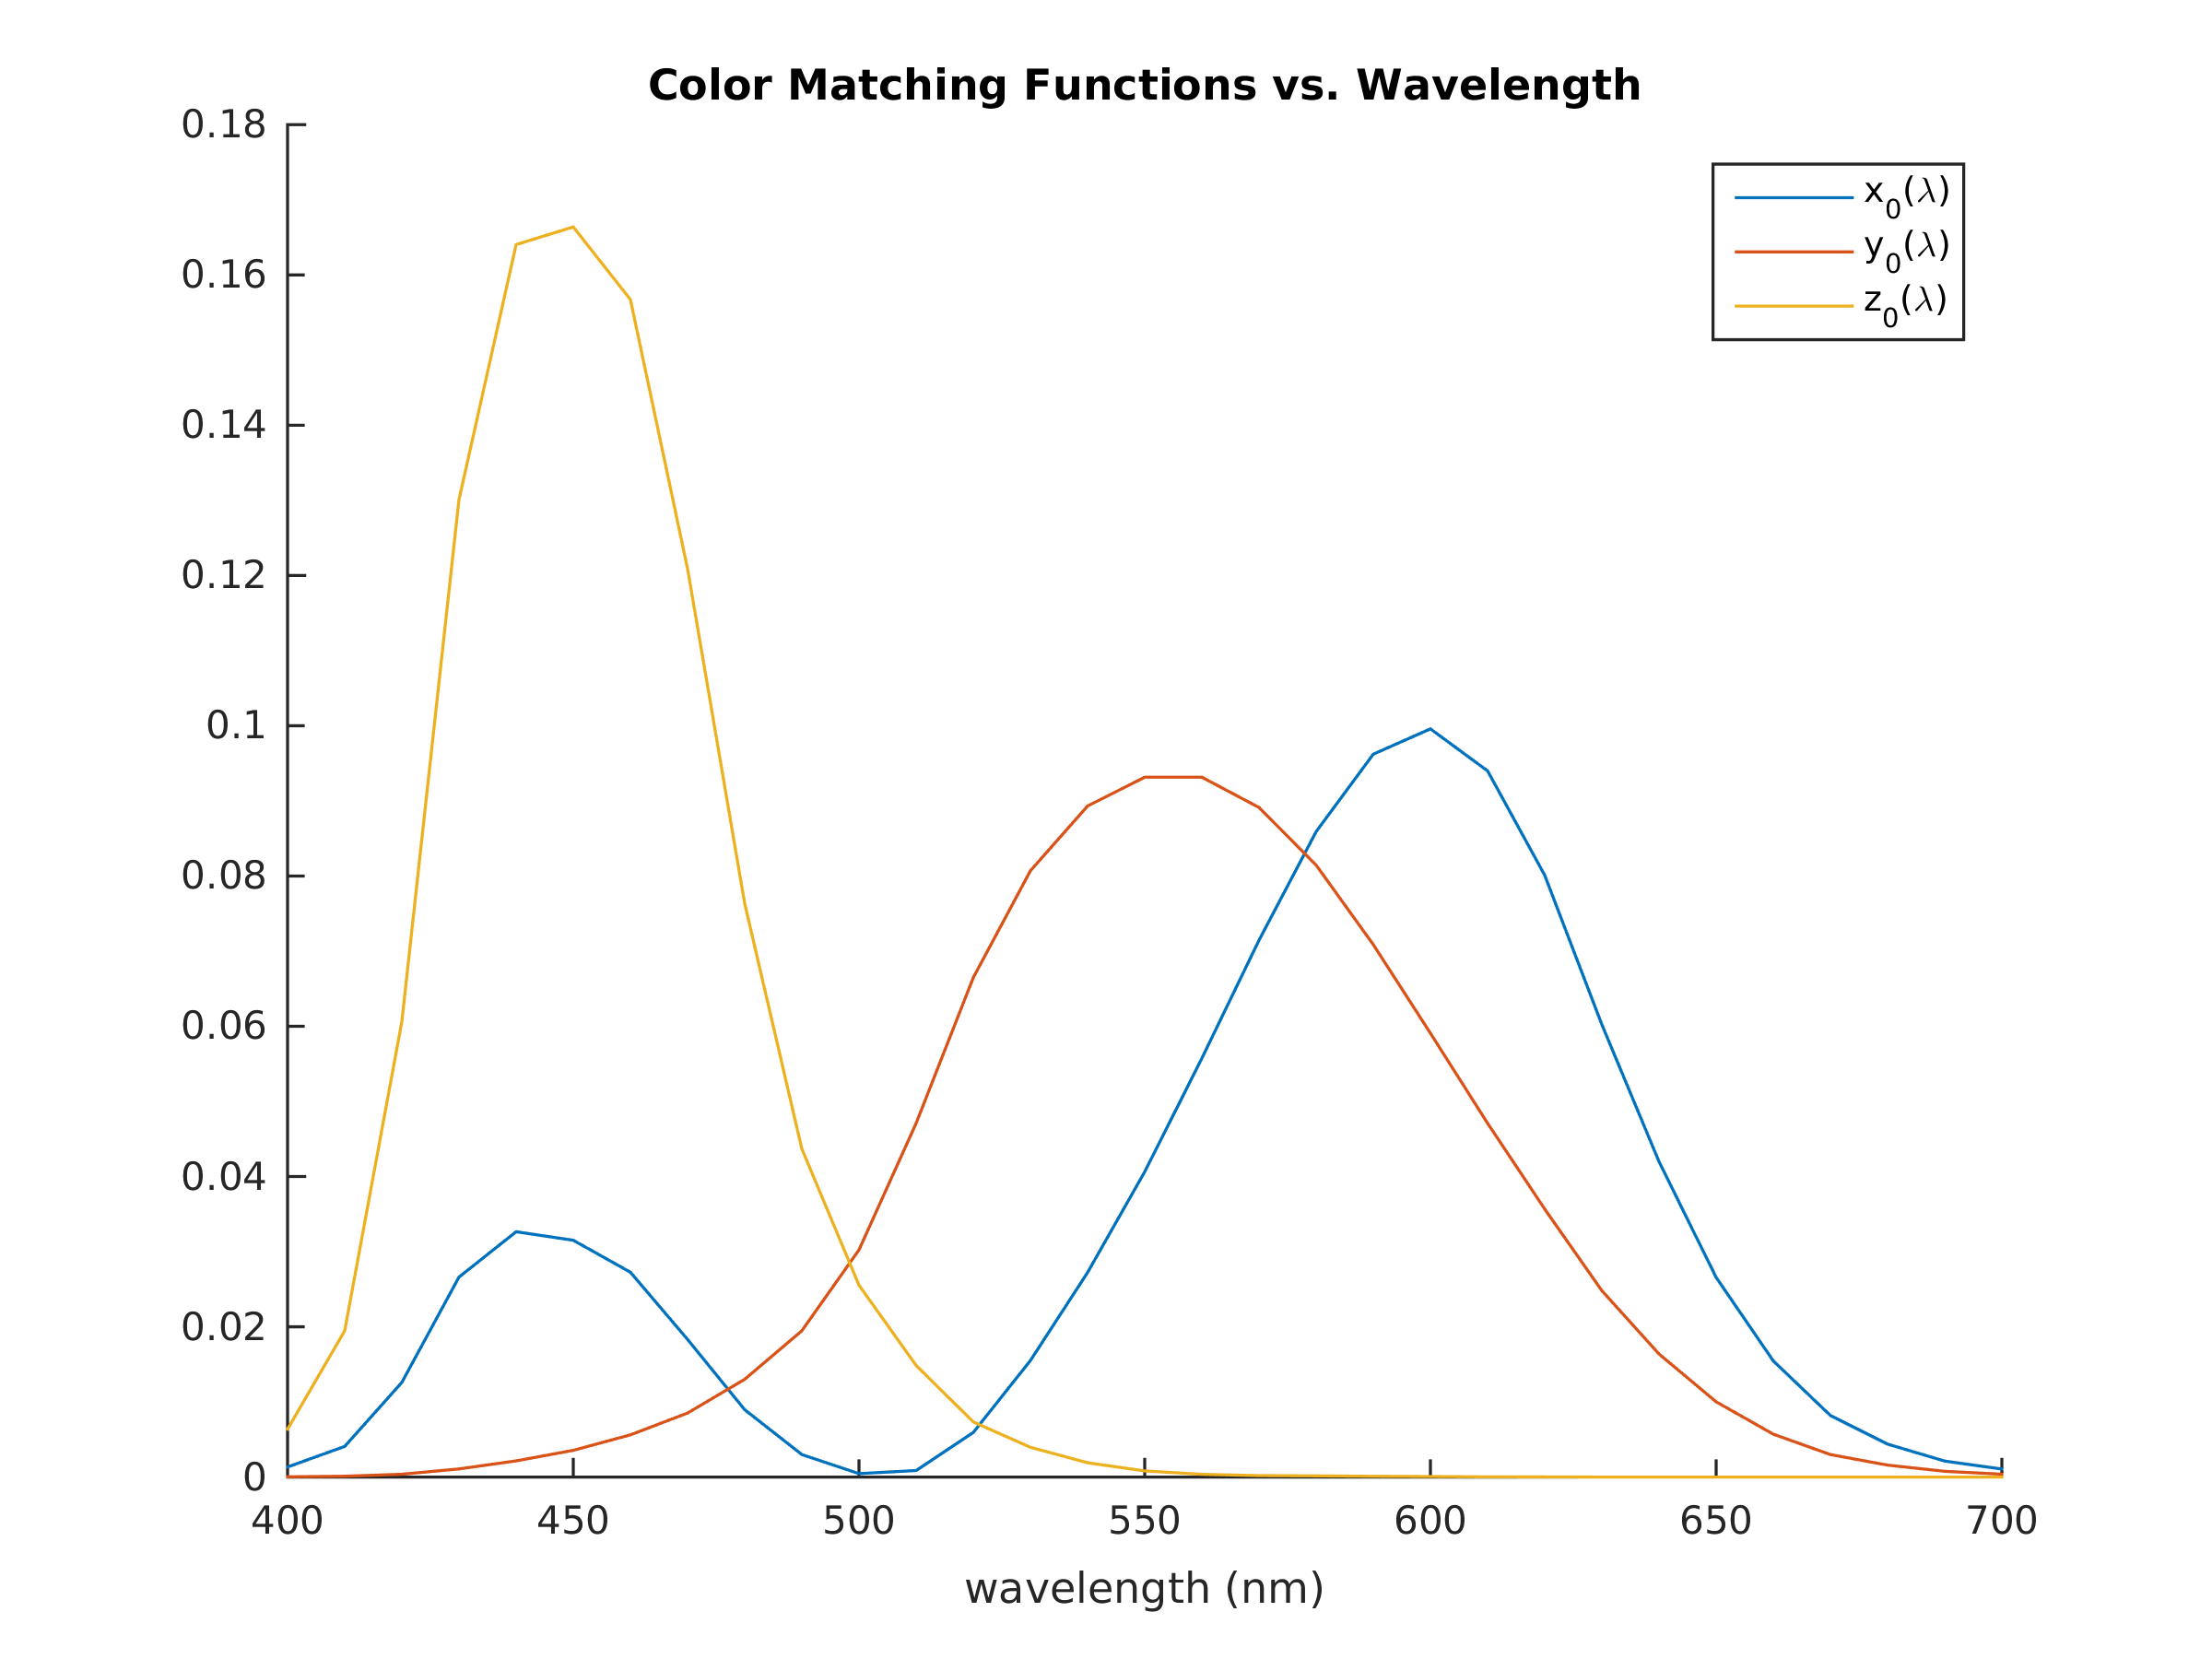
\includegraphics[width=0.6\textwidth]{xyzmatching.png}
			\caption{Color Matching Functions vs. Wavelength}
		\end{center}
	\end{figure}

\pagebreak

\subsection{Plot $l_{0}(\lambda)$, $m_{0}(\lambda)$, $s_{0}(\lambda)$ Color
			Matching Functions}
	\begin{figure}[h]
		\begin{center}
			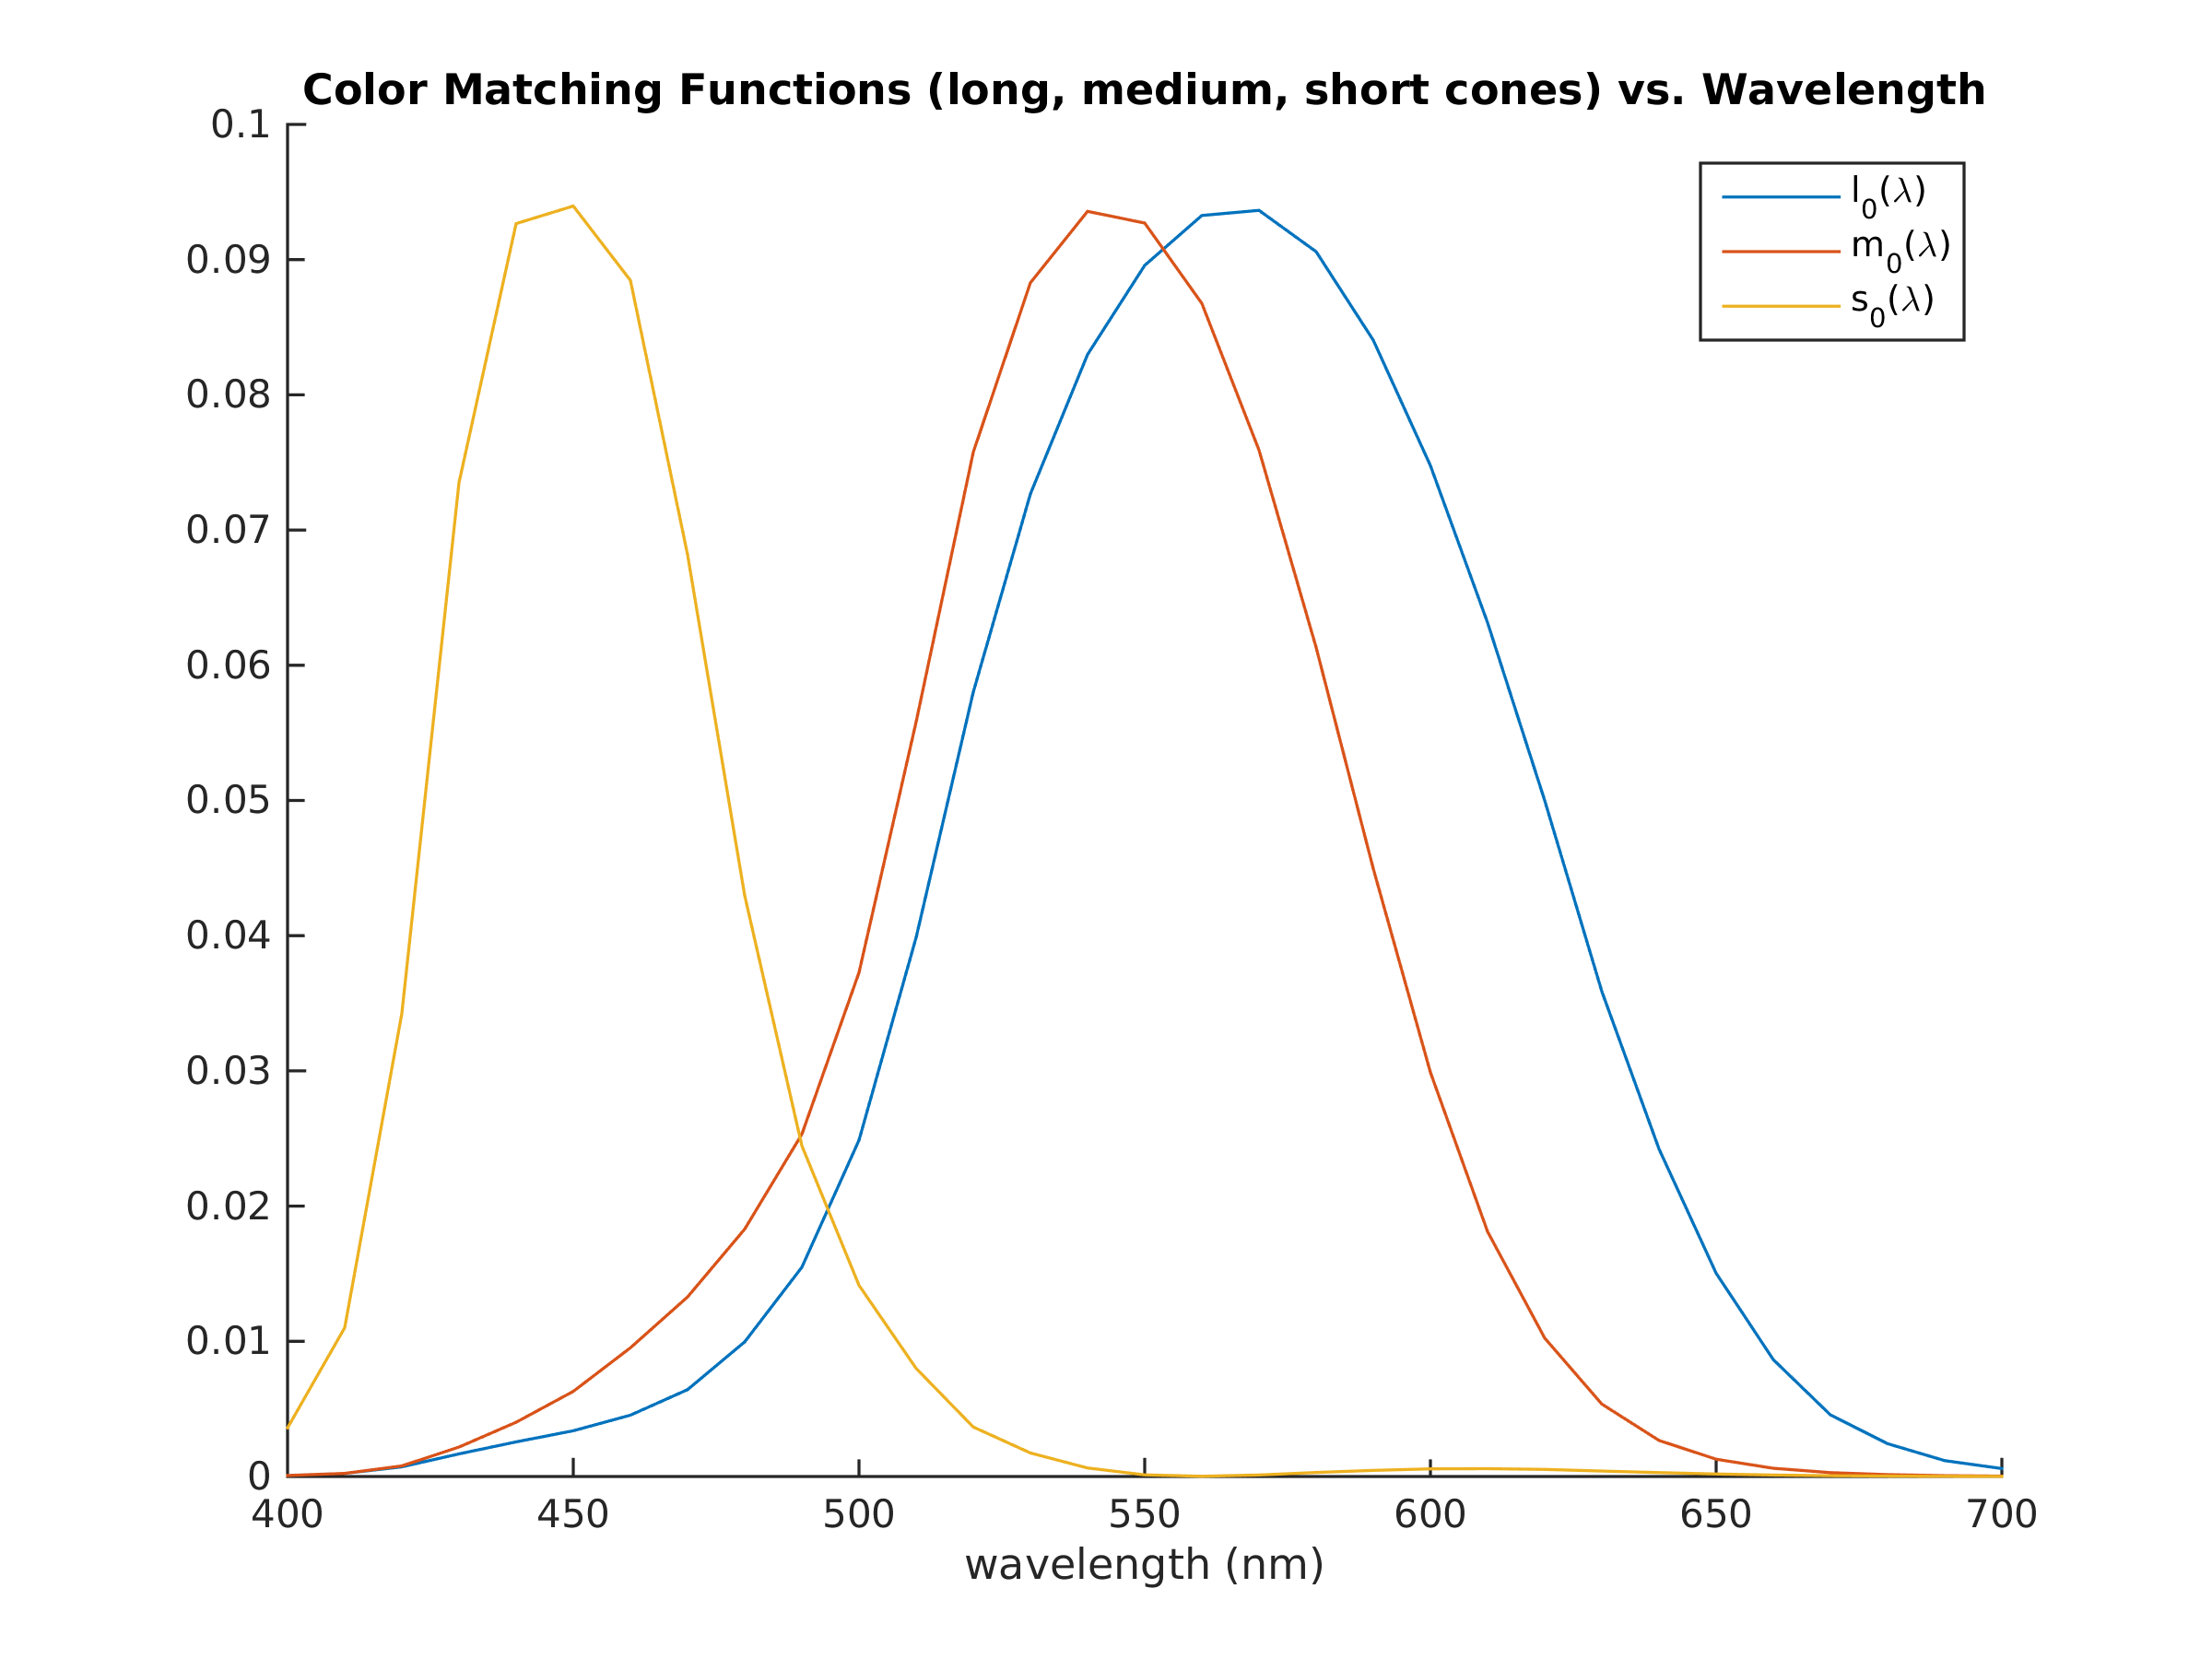
\includegraphics[width=0.6\textwidth]{lmnmatching.png}
			\caption{Color Matching Functions vs. Wavelength}
		\end{center}
	\end{figure}

\subsection{Plot $D_{65}$ and Fluorescent Illuminants}
	\begin{figure}[h]
		\begin{center}
			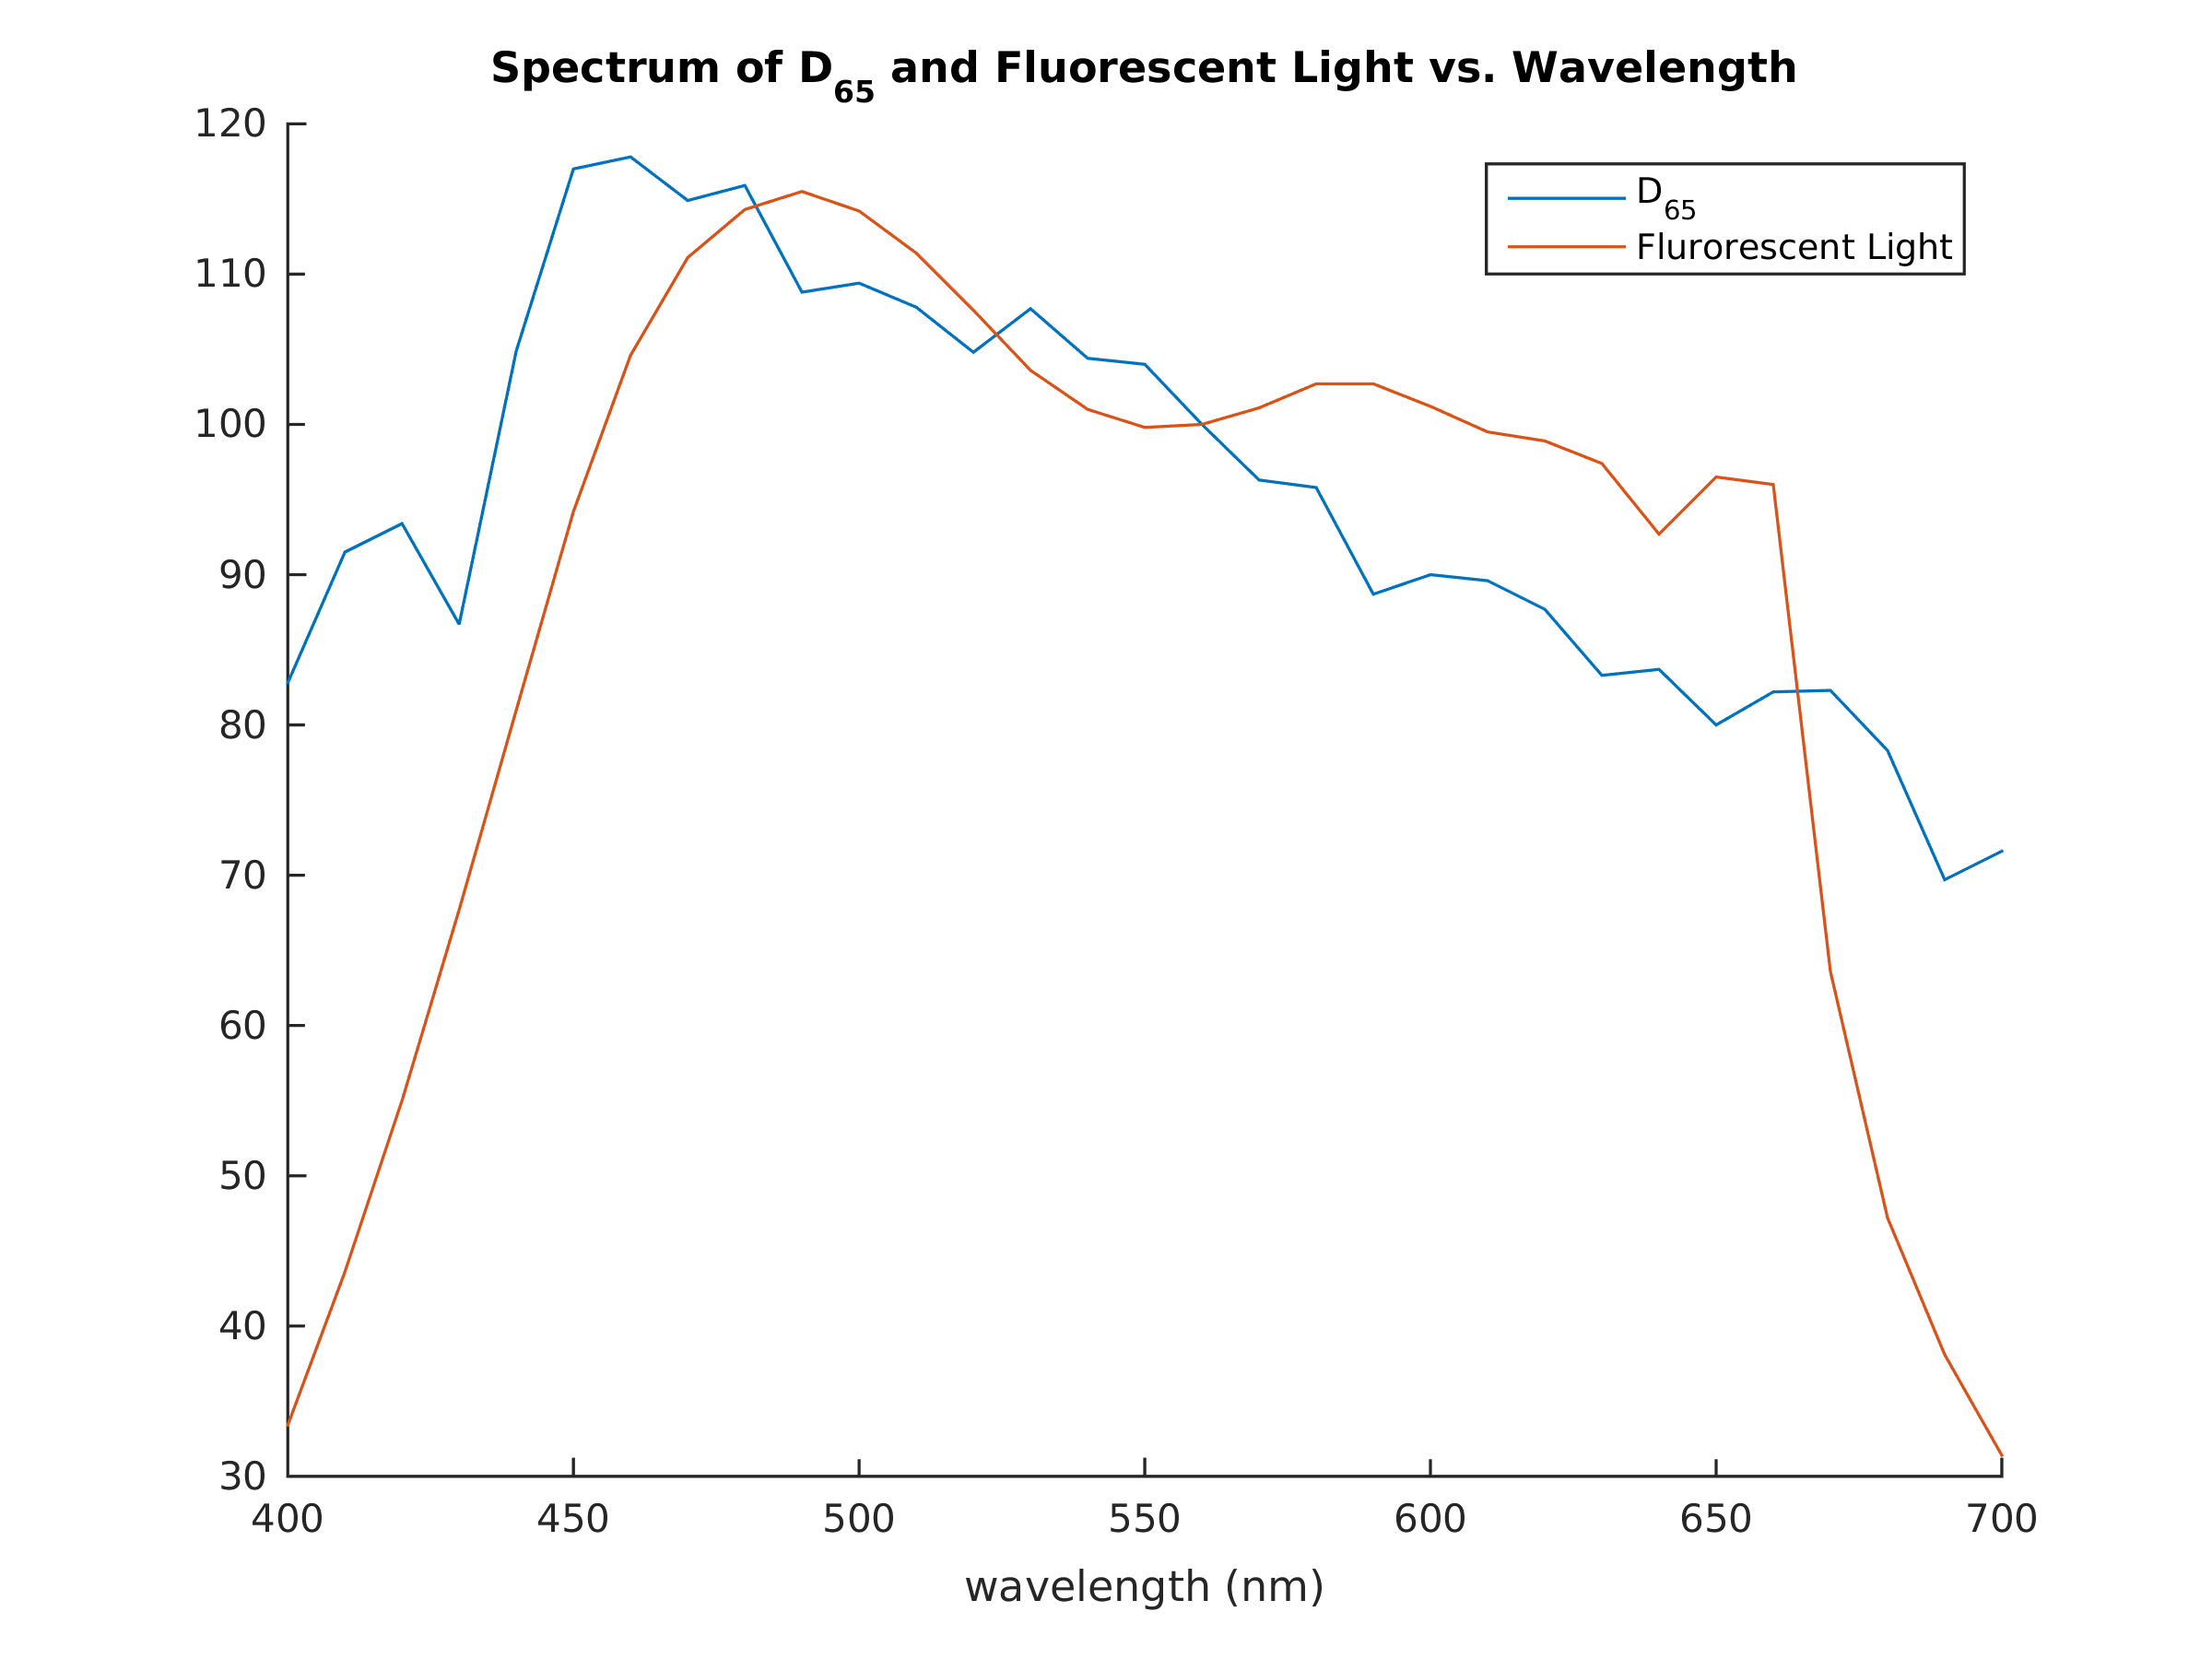
\includegraphics[width=0.6\textwidth]{illuminants.png}
			\caption{Spectrum of $D_{65}$ and Fluorescent vs. Wavelength}
		\end{center}
	\end{figure}

%----------------------------------------------------------------------------------------
%	SECTION 3
%----------------------------------------------------------------------------------------
\section{Chromaticity Diagrams}
	In this section, chromaticity diagrams are plotted using provided data.

\subsection{Plot Chromaticity Diagram}
	\begin{figure}[h]
		\begin{center}
			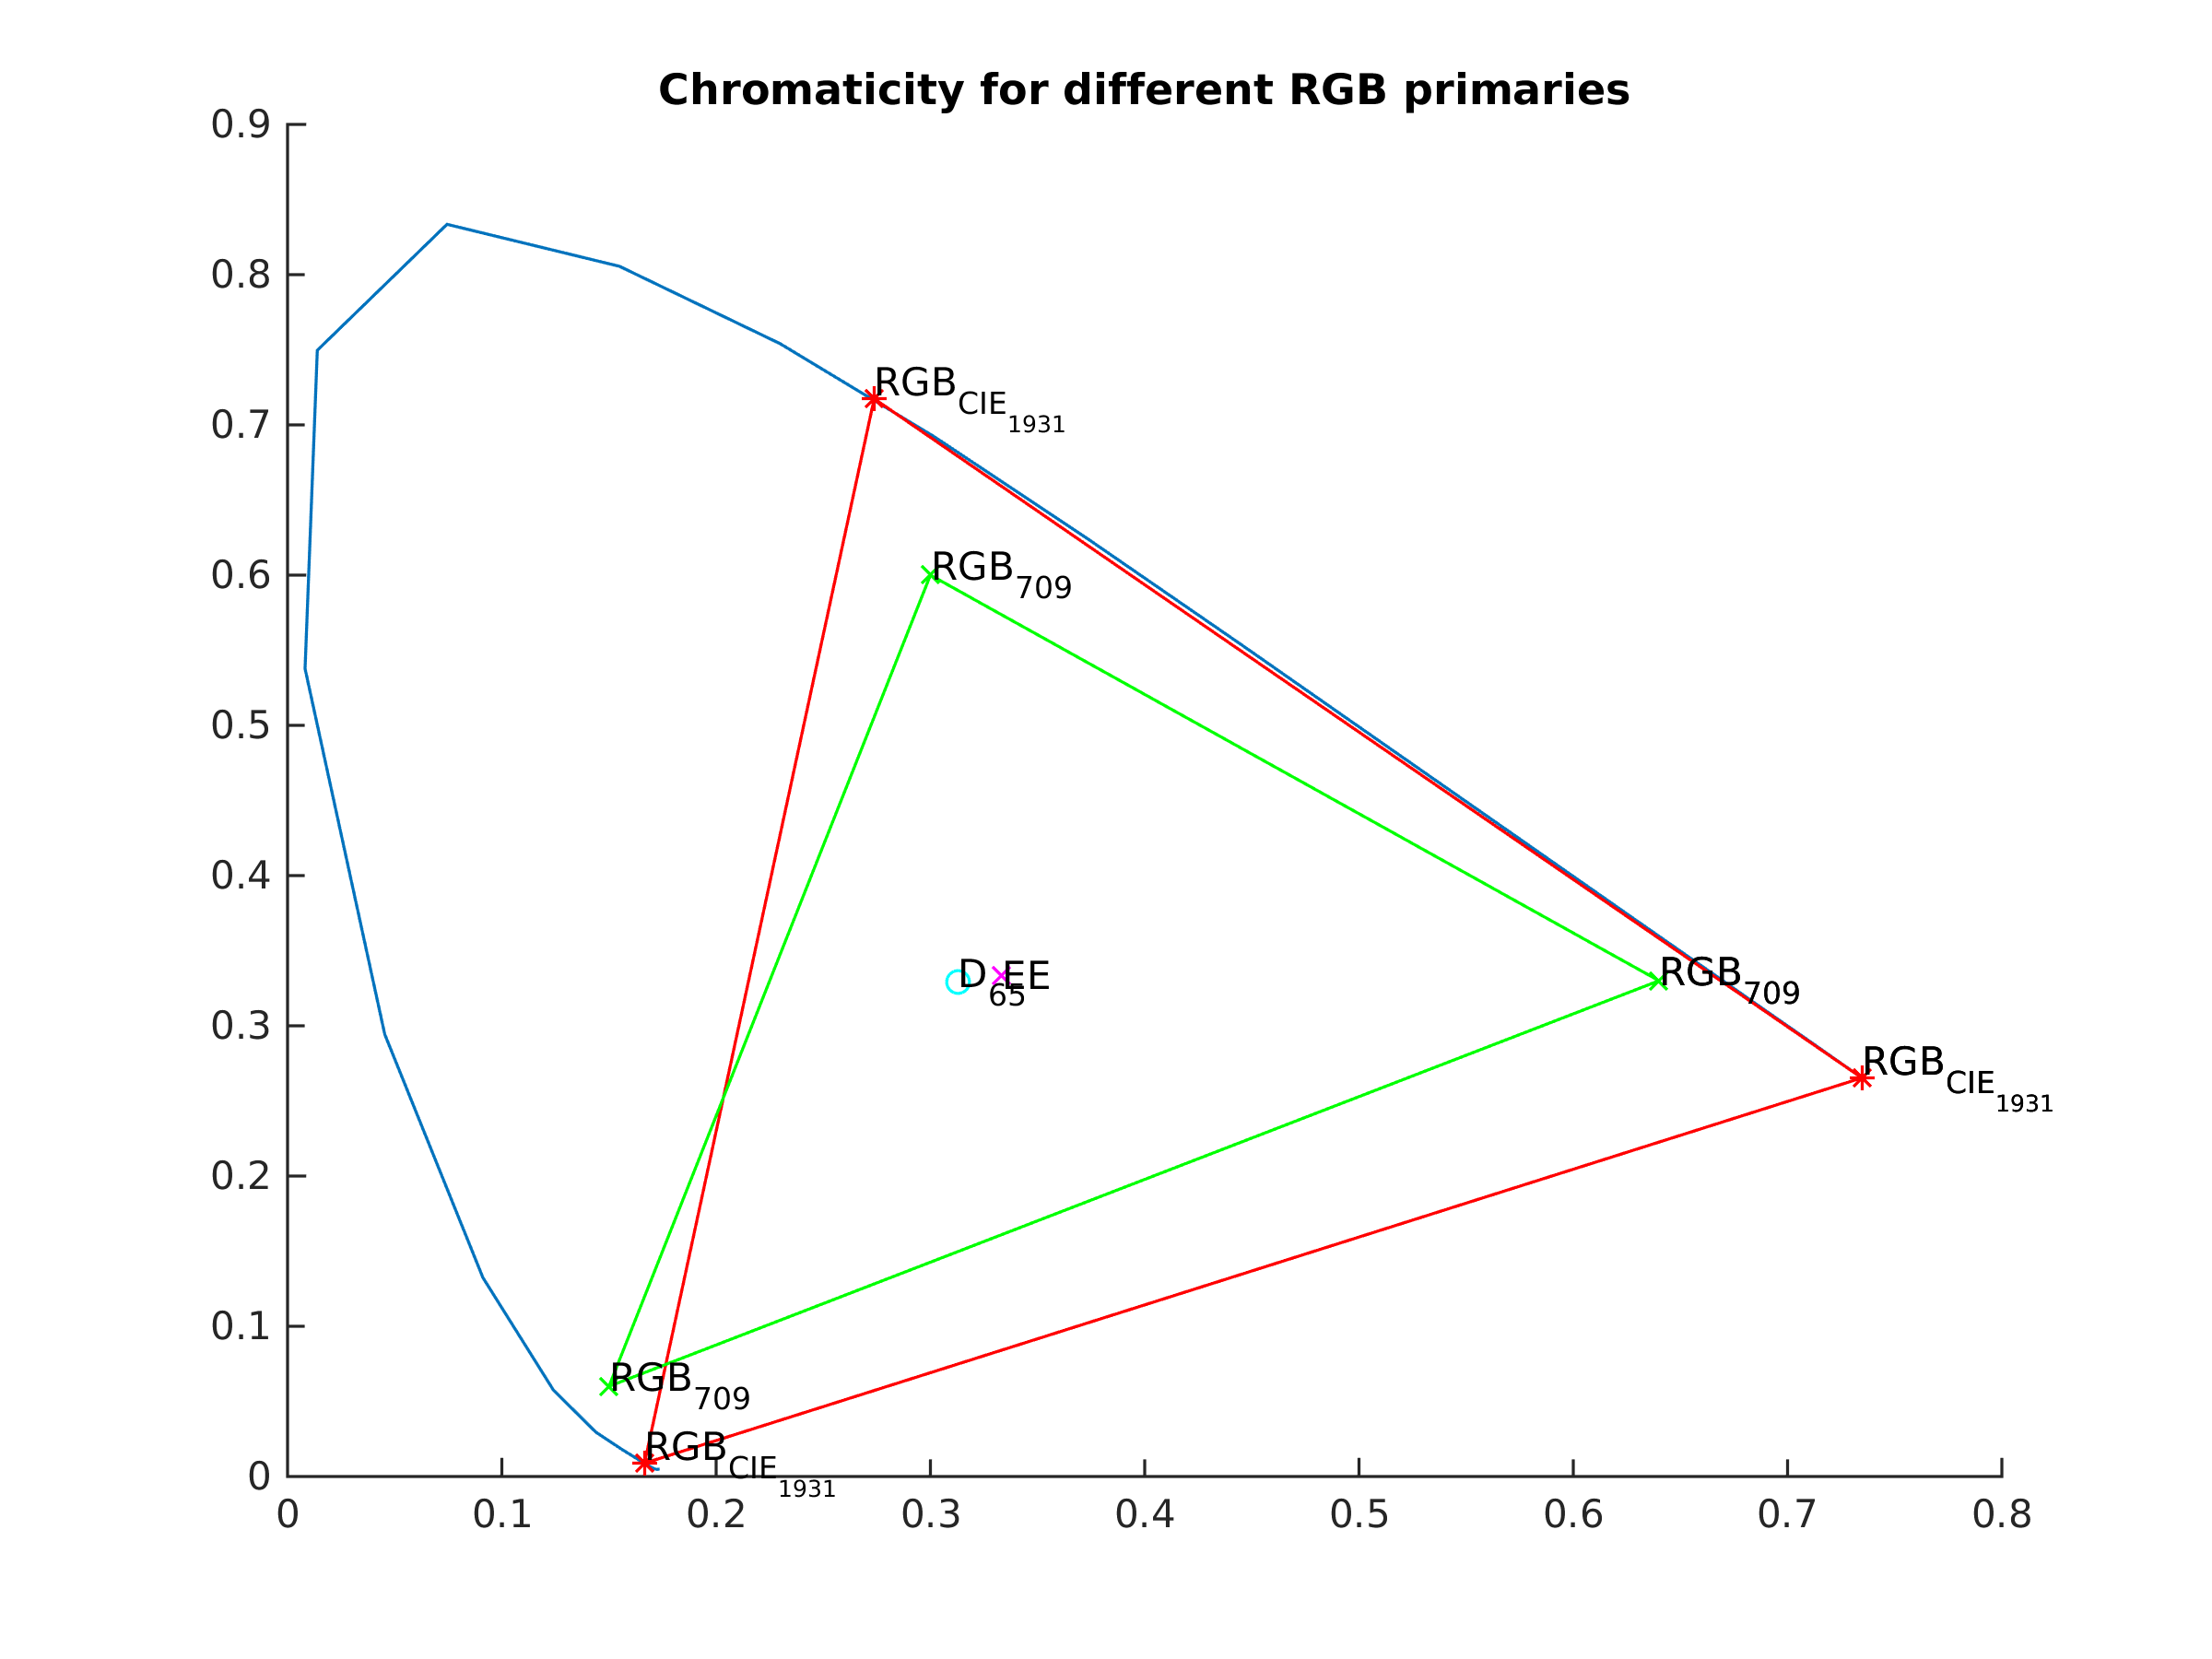
\includegraphics[width=0.6\textwidth]{chromaticity.png}
			\caption{Chromaticity Diagram}
		\end{center}
	\end{figure}

%----------------------------------------------------------------------------------------
%	SECTION 4
%----------------------------------------------------------------------------------------
\section{Rendering an Image from Illuminant, Reflectance, and Color Matching
		Functions}
	In this section, image data are loaded. The transformation matrix using
	Rec. 709 RGB primaries and $D_{65}$ white point is calculated. RGB
	coordinates are then computed using the $XYZ$ and transformation matrix $M$.
	The image is then gamma-corrected and plotted.

\subsection{Calculation of $M_{709D65}$}
	From equation (15) of the lab manual, we have:
	\begin{equation}
		M =
		\begin{bmatrix}
		x_r & x_g & x_b \\
		y_r & y_g & y_b \\
		z_r & z_g & z_b \\
		\end{bmatrix}
		\begin{bmatrix}
		\kappa_r & 0 & 0 \\
		0 & \kappa_g & 0 \\
		0 & 0 & \kappa_b \\
		\end{bmatrix}
	\end{equation}
	and from equation (17), we have:
	\begin{equation}
		\begin{bmatrix}
		\kappa_r \\
		\kappa_g \\
		\kappa_b \\
		\end{bmatrix}
		=
		\begin{bmatrix}
		x_r & x_g & x_b \\
		y_r & y_g & y_b \\
		z_r & z_g & z_b \\
		\end{bmatrix}
		^{-1}
		\begin{bmatrix}
		x_{wp}/y_{wp} \\
		1 \\
		z_{wp}/y_{wp}\\
		\end{bmatrix}
		.
	\end{equation}
	We also have:
	\begin{equation}
		\begin{bmatrix}
		x_r & x_g & x_b \\
		y_r & y_g & y_b \\
		z_r & z_g & z_b \\
		\end{bmatrix}
		=
		\begin{bmatrix}
		0.640 & 0.300 & 0.150 \\
		0.330 & 0.600 & 0.060 \\
		0.030 & 0.100 & 0.790 \\
		\end{bmatrix}
	\end{equation}
	and,
	\begin{equation}
		\begin{bmatrix}
		x_{wp} \\
		y_{wp} \\
		z_{wp} \\
		\end{bmatrix}
		=
		\begin{bmatrix}
		0.3127 \\
		0.3290 \\
		0.3583 \\
		\end{bmatrix}
		.
	\end{equation}
	Using (3) and (4), we have:
	\begin{align*}
		\begin{bmatrix}
		\kappa_r \\
		\kappa_g \\
		\kappa_b \\
		\end{bmatrix}
		=
		\begin{bmatrix}
		0.640 & 0.300 & 0.150 \\
		0.330 & 0.600 & 0.060 \\
		0.030 & 0.100 & 0.790 \\
		\end{bmatrix}
		^{-1}
		\begin{bmatrix}
		0.3127/0.3290 \\
		1 \\
		0.3583/0.3290 \\
		\end{bmatrix}
	\end{align*}
	Hence,
	\begin{align*}
		\begin{bmatrix}
		\kappa_r \\
		\kappa_g \\
		\kappa_b \\
		\end{bmatrix}
		=
		\begin{bmatrix}
		0.6444 \\
		1.1919 \\
		1.2032 \\
		\end{bmatrix}
	\end{align*}
	Finally,
	\begin{align*}
		M =
		\begin{bmatrix}
		0.4124 & 0.3576 & 0.1805 \\
		0.2126 & 0.7152 & 0.0722 \\
		0.0193 & 0.1192 & 0.9505 \\
		\end{bmatrix}
	\end{align*}

\subsection{Plot Images Obtained from $D_{65}$ and Fluorescent Light Sources}
	\begin{figure}[h]
		\begin{subfigure}{0.5\textwidth}
			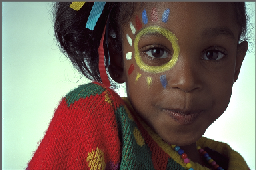
\includegraphics[width=0.9\textwidth]{gcimgd65.png}
		\end{subfigure}
		\begin{subfigure}{0.5\textwidth}
			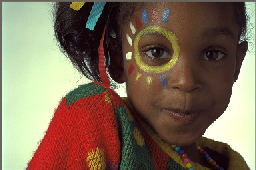
\includegraphics[width=0.9\textwidth]{gcimgflu.png}
		\end{subfigure}
		\caption{Images Obtained from $D_{65}$ and Fluorescent Light Sources}
	\end{figure}

\subsection{Qualitative Description of Two Images}
	The image obtained from the fluorescent light source is slightly brighter
	than than the image obtained from the $D_{65}$ light source.

\pagebreak
%----------------------------------------------------------------------------------------
%	SECTION 5
%----------------------------------------------------------------------------------------
\section{Color Chromaticity Diagram}

\subsection{Plot Color Diagram}
	\begin{figure}[h]
		\begin{center}
			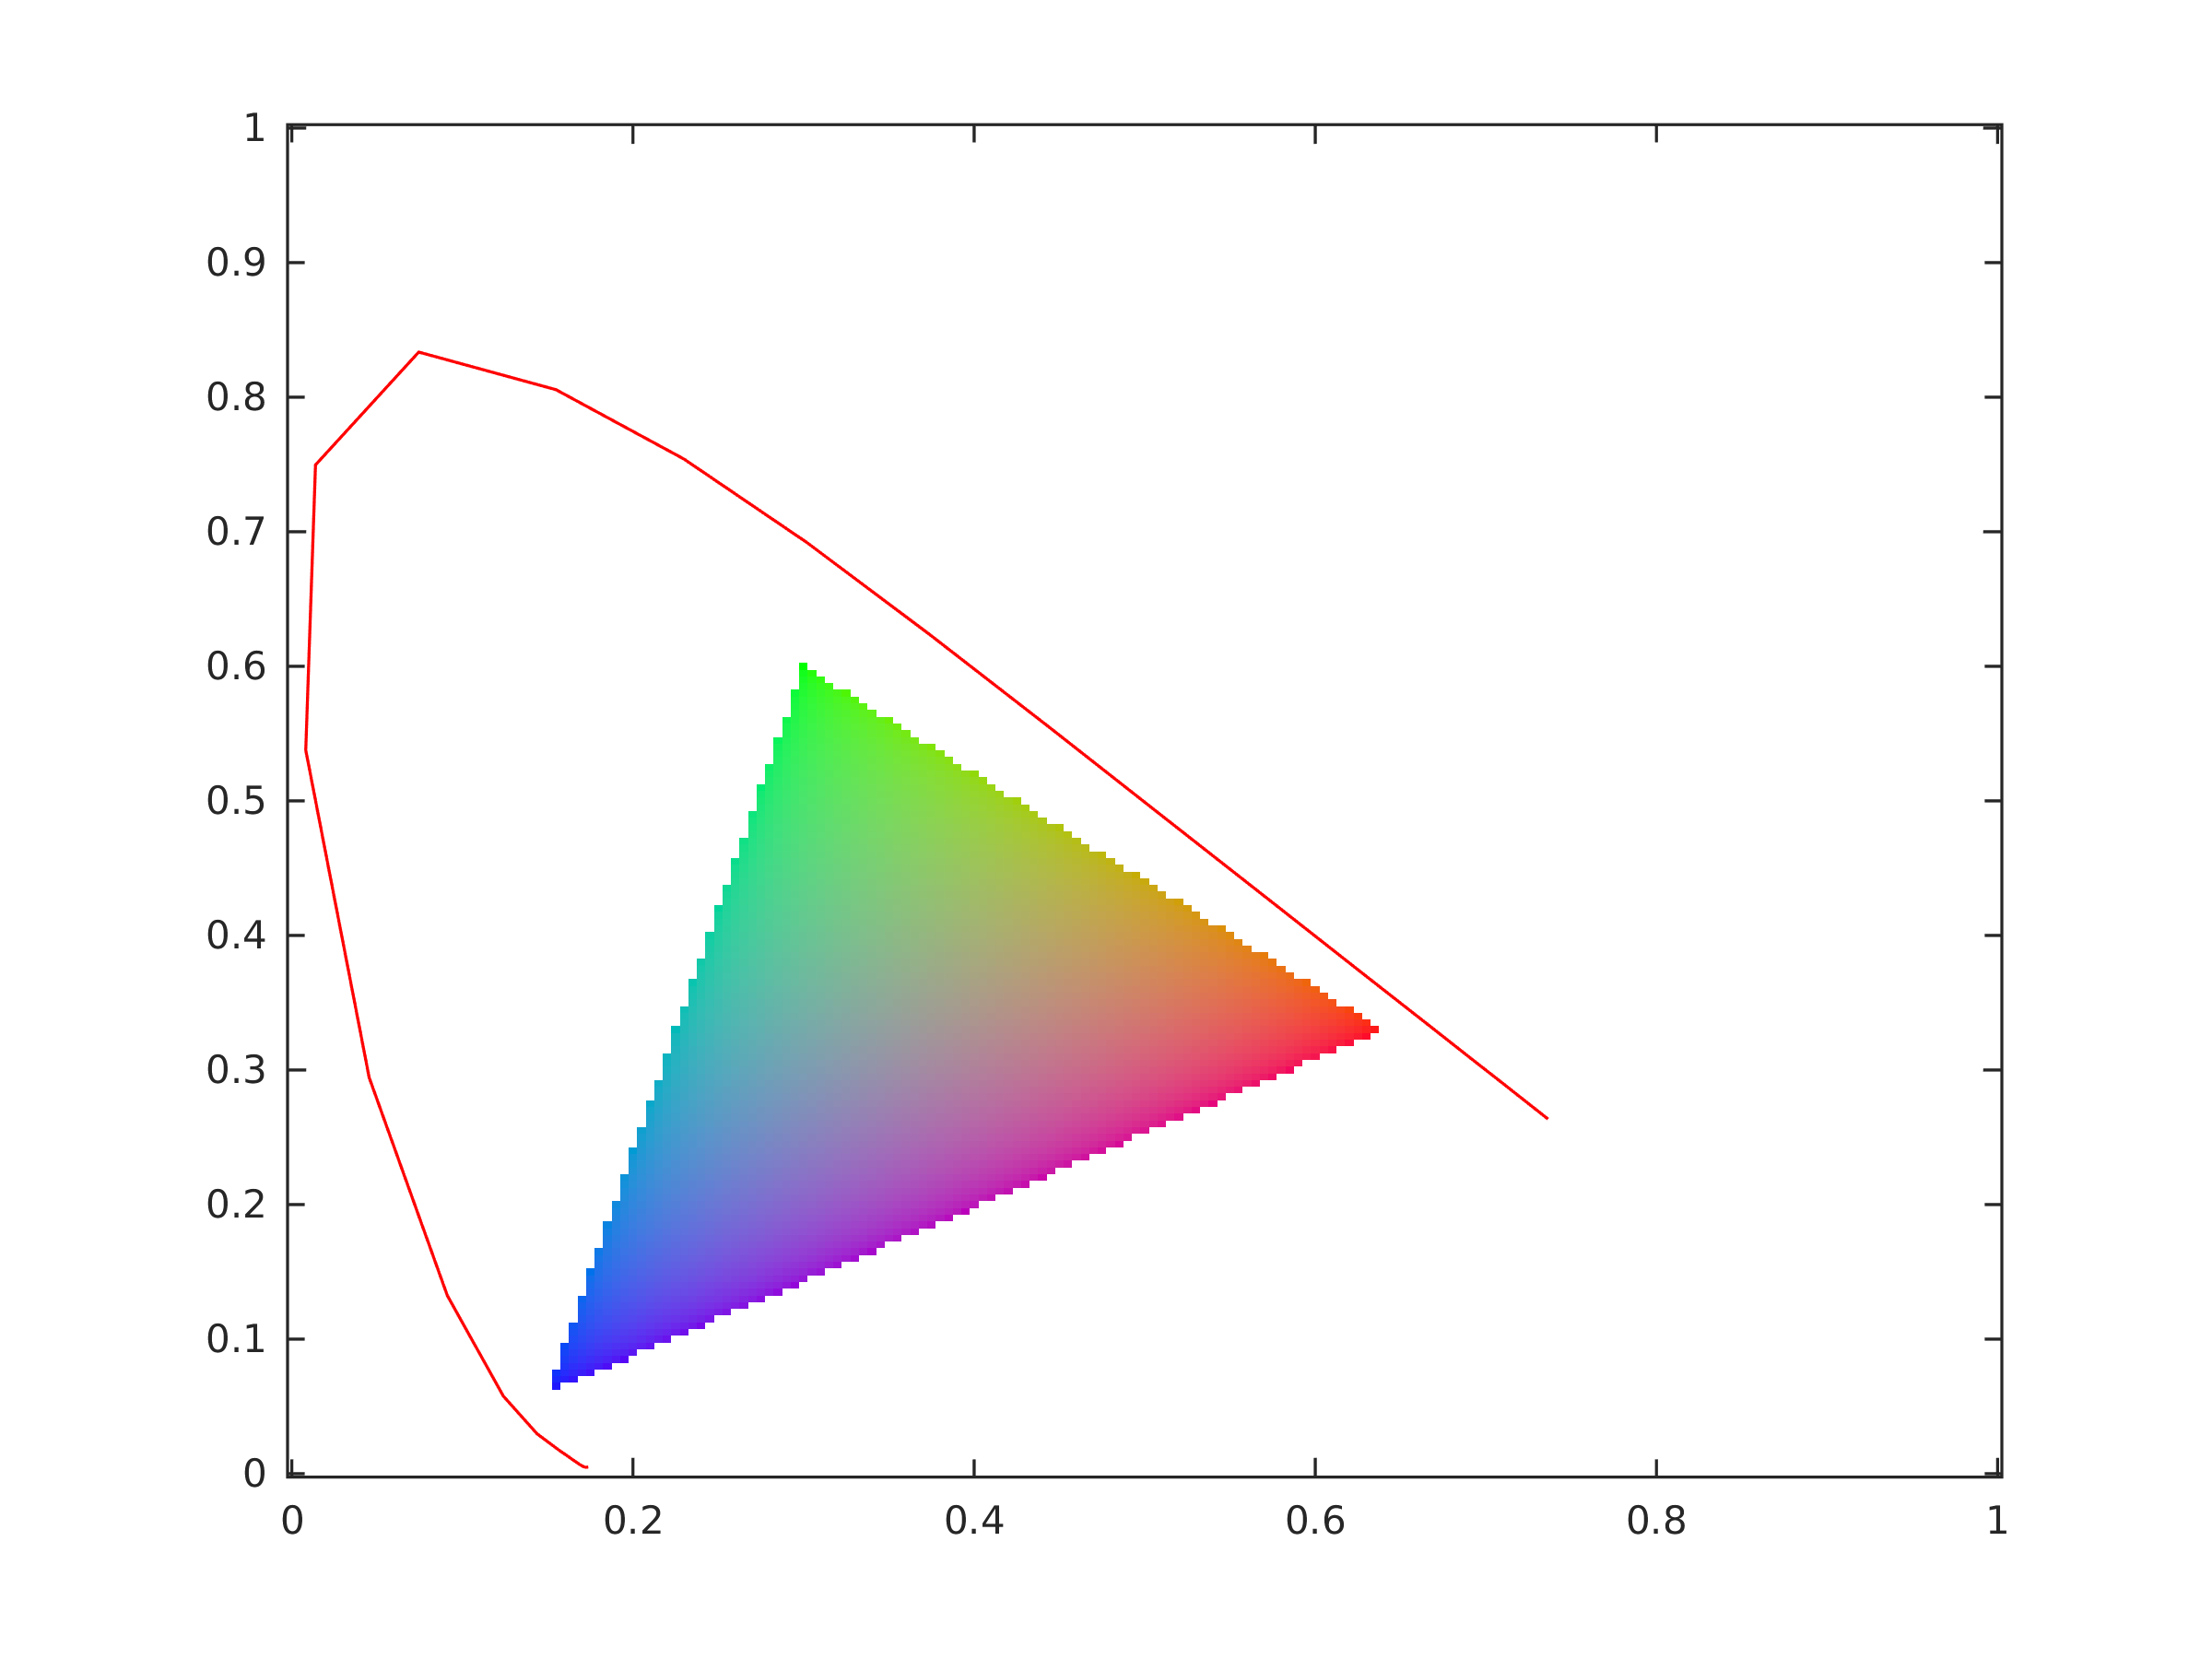
\includegraphics[width=0.6\textwidth]{color.png}
			\caption{Color Diagram}
		\end{center}
	\end{figure}

\end{document}
